% TEXINPUTS=.:$HOME/git/bvtex: latexmk  -pdf <main>.tex
\documentclass[xcolor=dvipsnames]{beamer}

\input{defaults}
\input{beamer/preamble}

\setbeamertemplate{navigation symbols}{}
% \setbeamertemplate{background}[grid][step=1cm]

\usepackage{multirow}
\usepackage{siunitx}
\usepackage{xmpmulti}
\usepackage[export]{adjustbox}
\usepackage{ulem}
\usepackage[outline]{contour}
\usepackage{pdfpages}
\usepackage{tikz}
\usetikzlibrary{shapes.geometric, arrows}
\usetikzlibrary{positioning}

\definecolor{bvtitlecolor}{rgb}{0.98, 0.92, 0.84}
\definecolor{bvoutline}{rgb}{0.1, 0.1, 0.1}

\renewcommand{\bvtitleauthor}{Brett Viren}
\renewcommand{\bvtit}{wc s/w}
\renewcommand{\bvtitle}{\LARGE Wire-Cell Software}
\renewcommand{\bvevent}{{\small DUNE S\&C @ BNL -- Jan 2019}}
\renewcommand{\bvdate}{Jan 2019}
\renewcommand{\bvbeamerbackground}{}

\def\Put(#1,#2)#3{\leavevmode\makebox(0,0){\put(#1,#2){#3}}}

\begin{document}
\input{beamer/title.tex}
\input{beamer/toc.tex}

\section{Wire-Cell Software Overview}

\begin{frame}
  \frametitle{Wire-Cell Algorithms and Processing Chain}

  %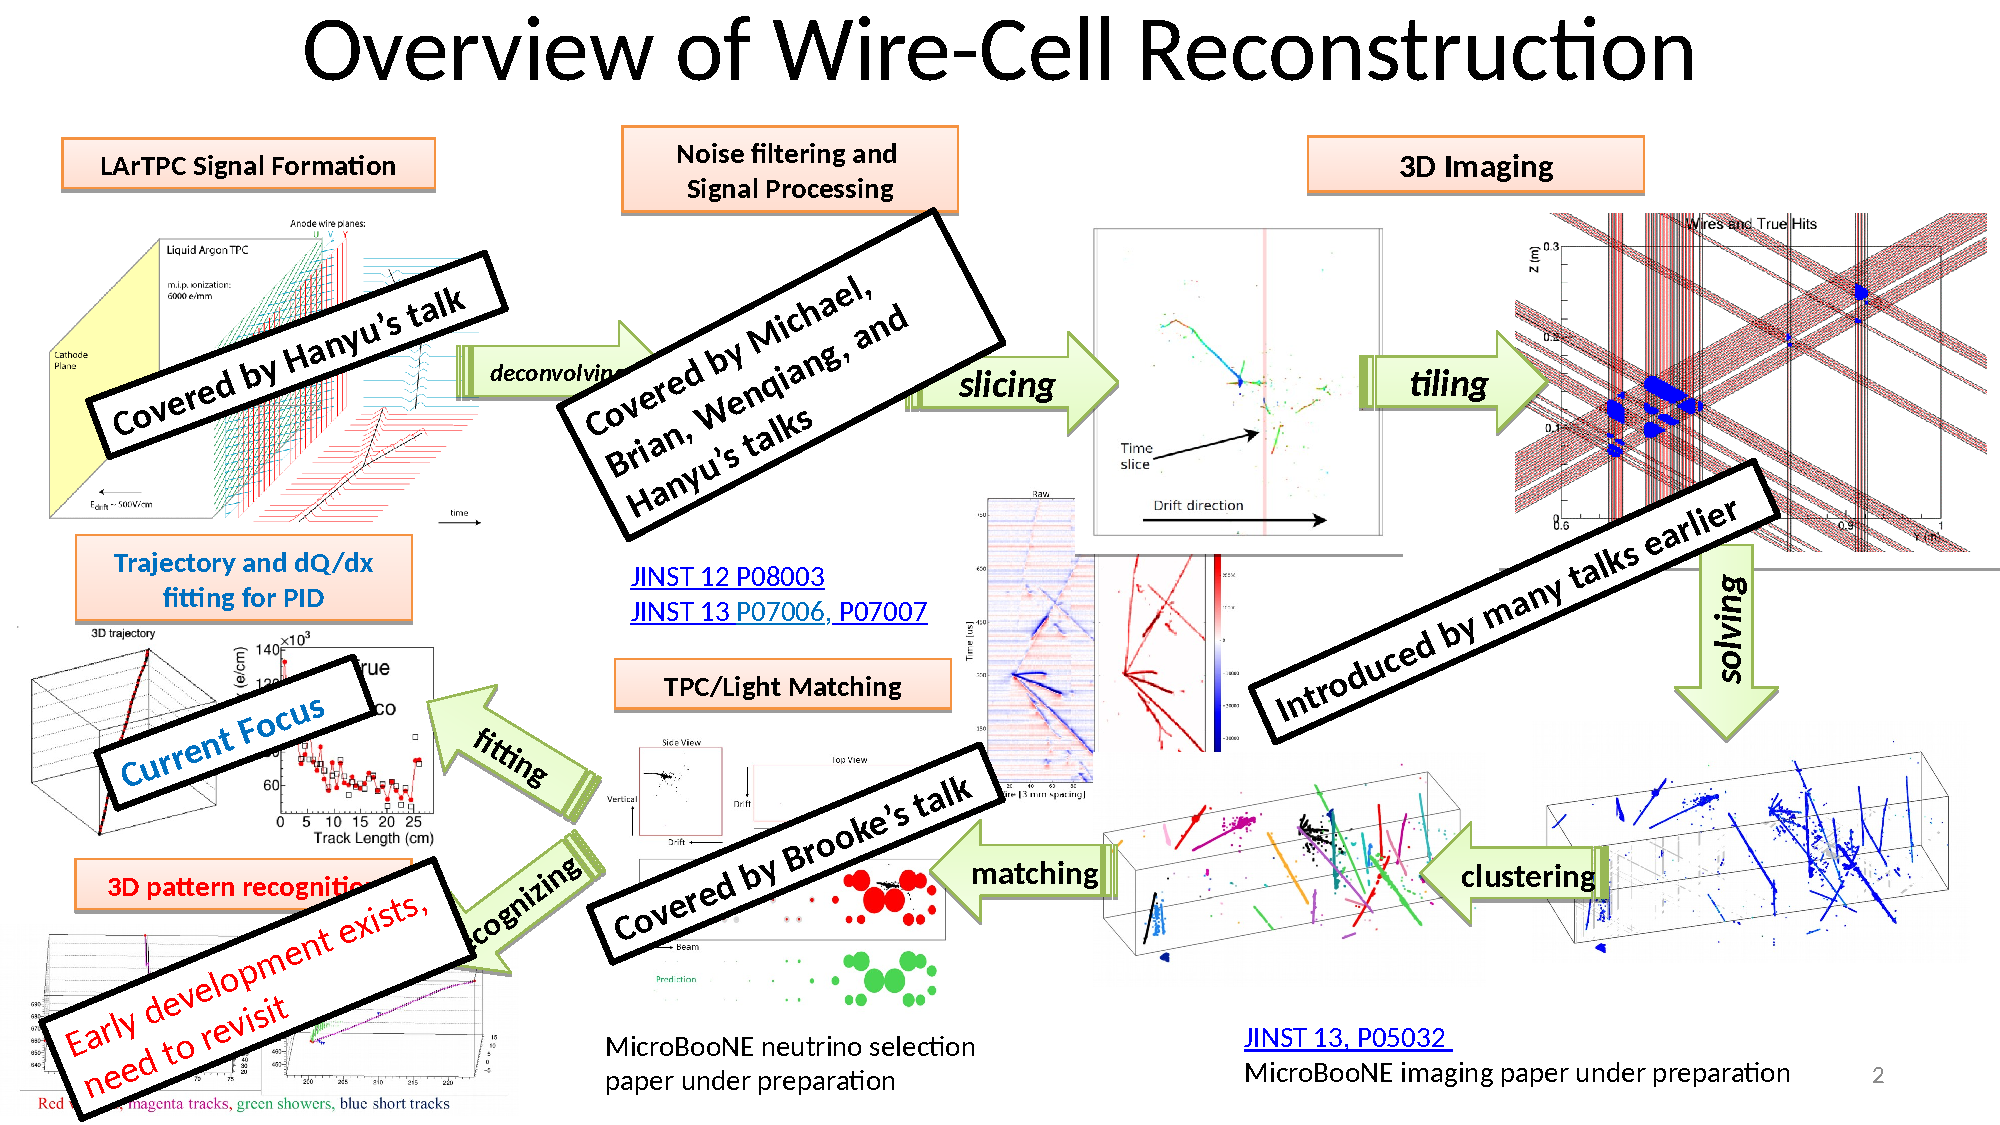
\includegraphics[width=\textwidth,clip,trim=0 0 0 2cm]{xin-wc-overview.pdf}
  \begin{center}
    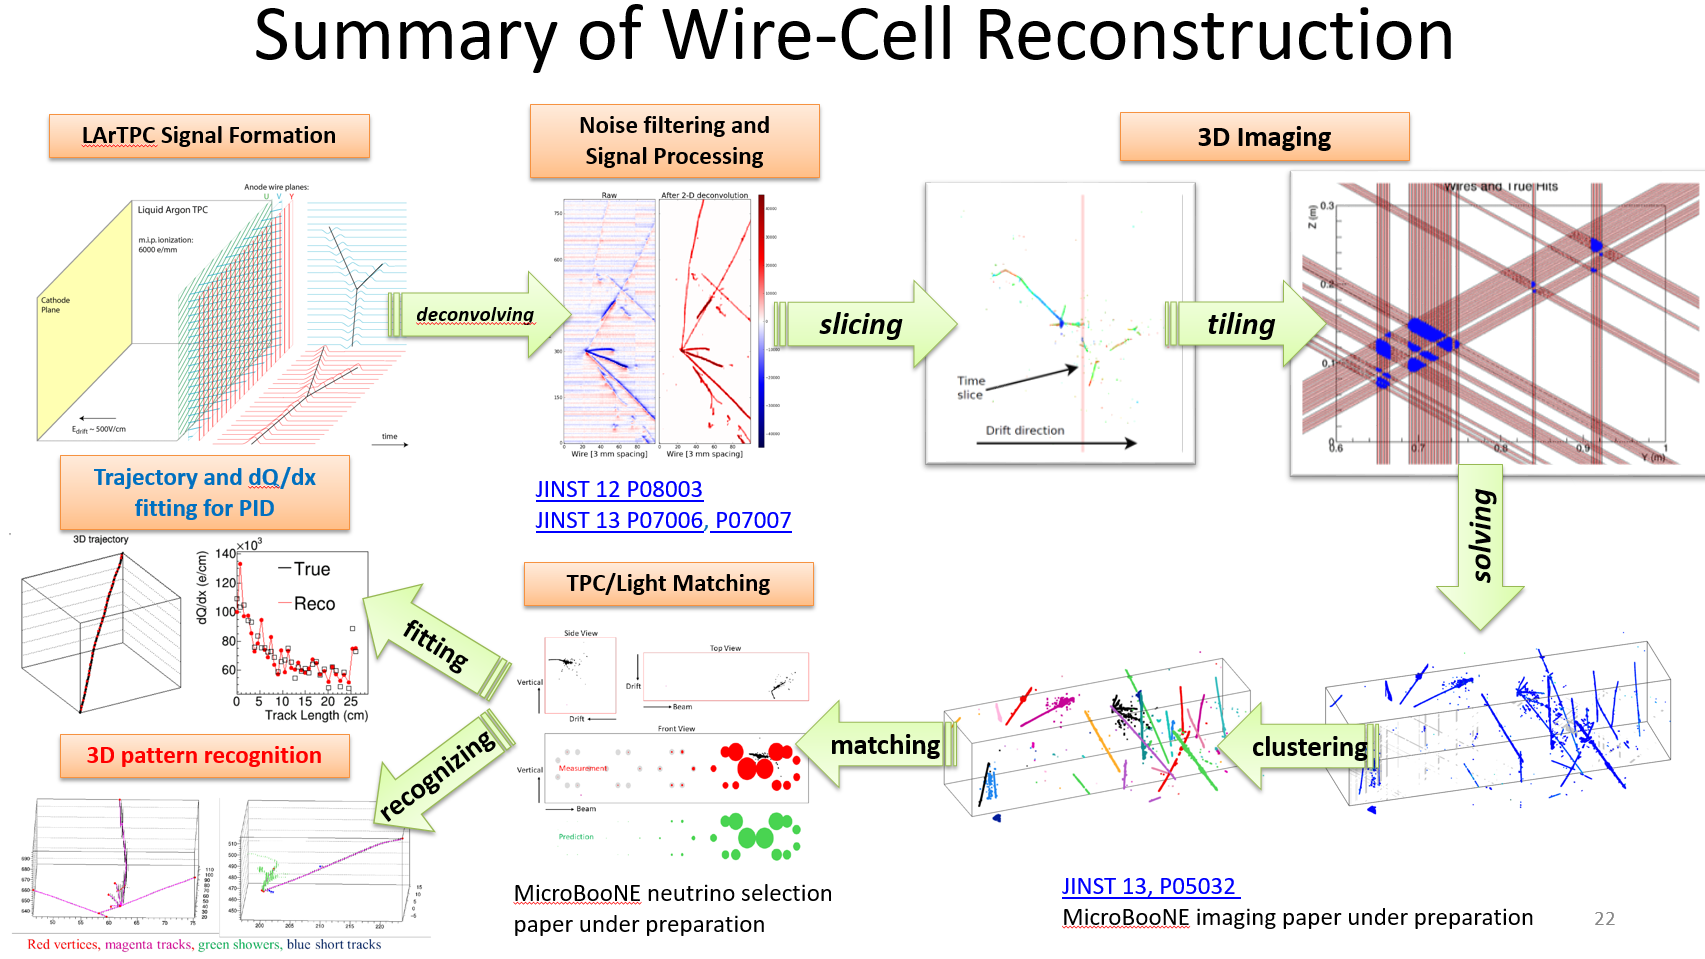
\includegraphics[width=\textwidth,clip,trim=0 0 0 3cm]{summary-of-wc-reco-noboxes.png}

    \tiny Xin Qian
  \end{center}

\end{frame}

\begin{frame}
  \frametitle{Wire-Cell Software Algorithm Scope}
  \begin{center}
  \includegraphics[height=0.9\textheight]{feature-scope.pdf}    
  \end{center}
\end{frame}


\begin{frame}
  \frametitle{Prototype and Toolkit Code Bases}
  Common:
  \begin{itemize}\footnotesize
  \item Similar build systems and external dependencies.
  \item Open source repositories on GitHub.
  \end{itemize}
  Prototype:
  \begin{itemize}\footnotesize
  \item Lightly structured code base, various \texttt{main()} programs, freedom to experiment without many ``rules'', comes with ``no'' user support, no releases.
    Initial proving ground for eventual toolkit code.
  \item Used by MicroBooNE results.
  \item Top package: \url{https://github.com/BNLIF/wire-cell}
  \end{itemize}
  Toolkit:
  \begin{itemize}\footnotesize
  \item Structured/designed code base, careful dependency control, toolkit-style integration to user's app, shared library plugins, configuration subsystem, optimized code, production releases and support.
  \item Used by MicroBooNE and ProtoDUNE.
  \item Top package: \url{https://github.com/wirecell/wire-cell-build}
  \end{itemize}
\end{frame}


\section{Wire-Cell Toolkit}
\begin{frame}
  \tableofcontents[currentsection,hideothersubsections]
\end{frame}


\begin{frame}
  \frametitle{Wire-Cell Toolkit Packages}
  \begin{description}\footnotesize
  \item[\texttt{util}] fundamental data types, operations, toolkit infrastructure.
  \item[\texttt{iface}] abstract ``interface'' base classes for WCT components.
  \item[\texttt{cfg}] reference configuration files (\texttt{.jsonnet} and \texttt{.fcl})
  \item[\texttt{data}] larger config ``data'' files (\texttt{.json.bz2})
  \item[\texttt{gen}] components for electron drift and field response signal and noise simulation.
  \item[\texttt{sigproc}] components for noise filtering and signal processing (field response deconvolution and L1 regularization)
  \item[\texttt{sio}] components to provide various I/O (depends on ROOT).
  \item[\texttt{python}] utility, debugging, analysis, config data file prep.
  \item[\texttt{pgraph}] single-thread, low-memory execution model implementation.
  \item[\texttt{tbb}] experimental multi-threaded execution model implementation.
  \item[\texttt{sing}] Singularity image creation and user scripts.
  \item[\texttt{docs}] news blog, manual, presentations and other documentations.
  \item[\texttt{tests}] larger-than-unit tests
  \item[\texttt{waftools}] build system support.
  \end{description}
\end{frame}

\begin{frame}
  \frametitle{Layered stack of user-code entry points}

  \begin{center}
    {\renewcommand{\arraystretch}{1.5}%
    \begin{tabular}[h]{|c|c|} \hline
      \texttt{wire-cell} CLI & \texttt{art} CLI \\
      & Wire-Cell/LArSoft integration \\
      \hline
      \hline
      \multicolumn{2}{|c|}{Wire-Cell plugin/shared libraries} \\
      \hline
      \hline
      \multicolumn{2}{|c|}{construct data flow processing graph via user configuration} \\
      \hline
      \multicolumn{2}{|c|}{use abstract component interfaces via factory lookup}\\
      \hline
      \multicolumn{2}{|c|}{\texttt{\#include "implementation.h"} / use concrete WC classes}\\
      \hline
      \multicolumn{2}{|c|}{implement new concrete component classes} \\
      \hline
      \multicolumn{2}{|c|}{design new interface base classes} \\
      \hline
    \end{tabular}}
  \end{center}
\end{frame}

\begin{frame}
  \frametitle{Aside: Data Flow Programming Paradigm}
  \footnotesize Programming = drawing: construct a \textbf{directed graph} of processing \textbf{nodes} with labeled \textbf{ports} connected by \textbf{edges} which transfer data objects.

  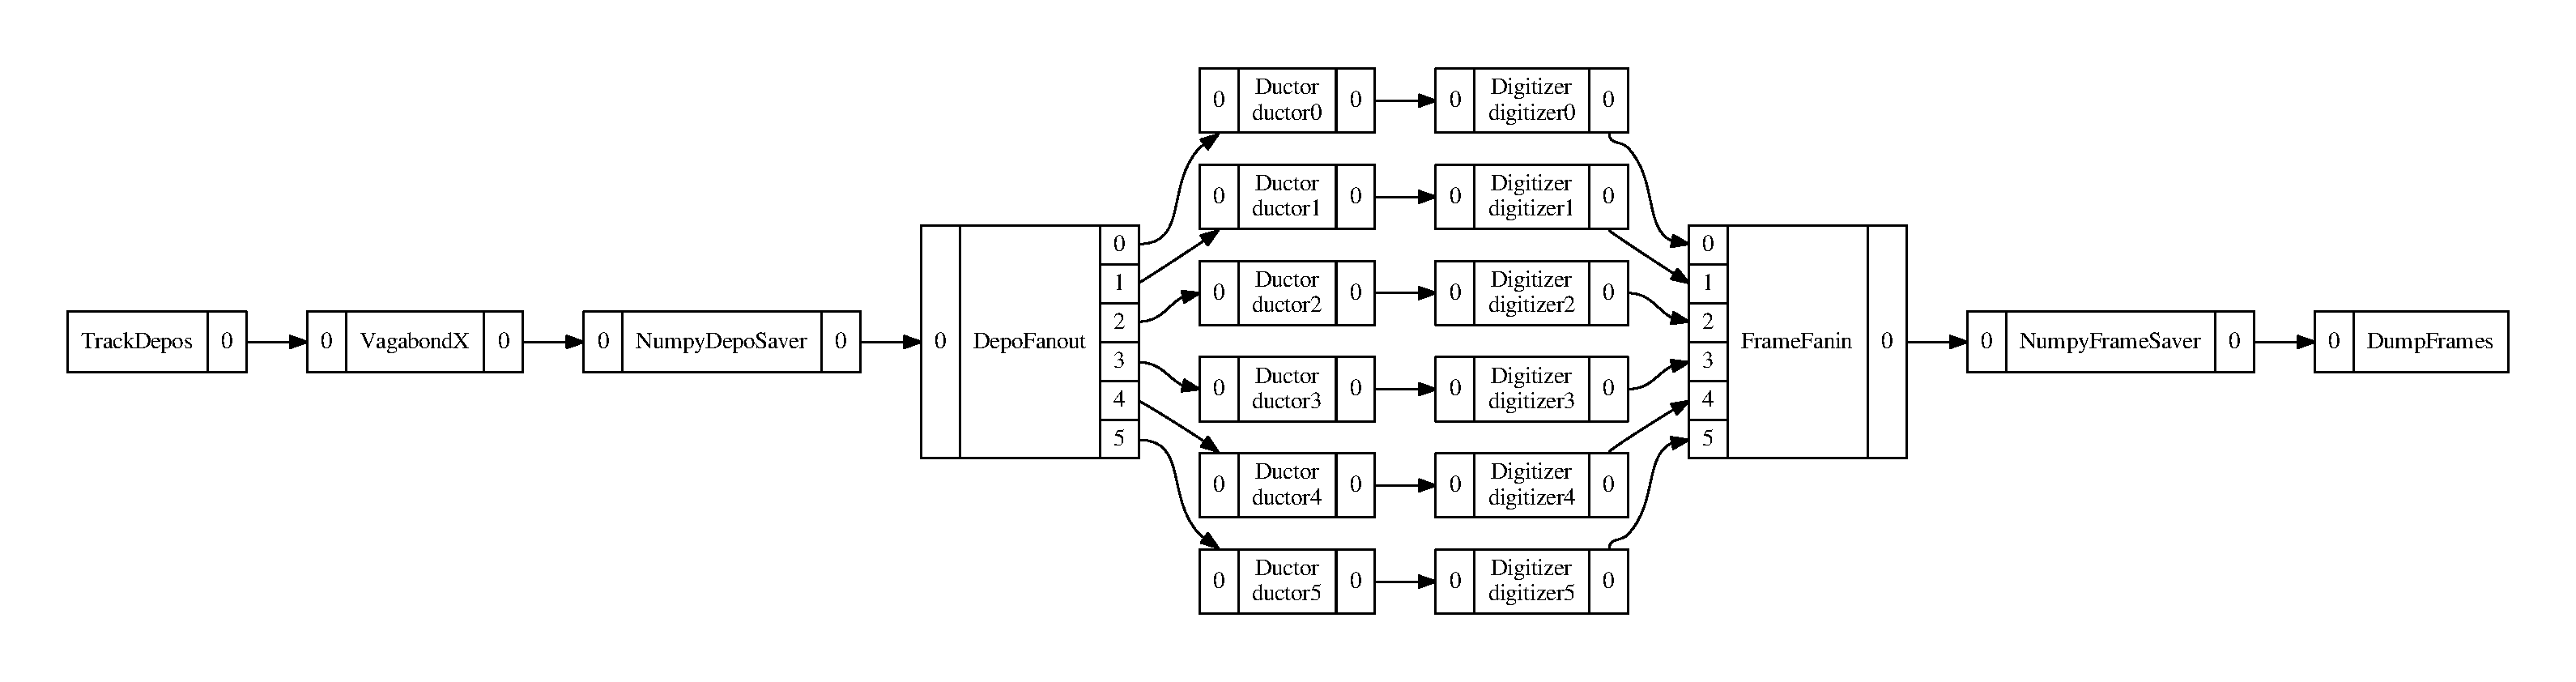
\includegraphics[width=\textwidth]{test-multiapa.pdf}
  
  \begin{itemize}\scriptsize
  \item Nodes may contain state, edges may buffer intermediate results.
  \item Stateless nodes and thread-safe edges allow for multi-threading.
  \item Edges may be generalized to allow multi-node communication. 
  \item Edge data may be fine-grained (ie, objects smaller than one ``event'').
  \item Different graph execution strategies may be employed.
  \end{itemize}

\end{frame}

\begin{frame}
  \frametitle{WCT Implements DFP Paradigm}
  \begin{itemize}\footnotesize
  \item Technically optional but all ``real'' jobs defined in terms of a DFP graph.
  \item WCT Jsonnet configuration supports \textbf{scale invariant} graph construction.
    \begin{itemize}\scriptsize
    \item[o] Complex subgraph description can be encapsulated into a single node object, parameterized and re-used.
    \end{itemize}

  \item Abstracted graph execution supports different execution strategies:
    \begin{itemize}\scriptsize
    \item[o] Primary engine: single-thread with memory-minimizing.
    \item[o] Experimental: TBB-based multi-threaded, CPU-maximizing.
    \item[o] Possible future: multi-thread+multi-node with ZeroMQ or MPI?
    \end{itemize}
  \end{itemize}
  
\end{frame}

\section{WC/LS/\textit{art} Integration}
\begin{frame}
  \tableofcontents[currentsection,hideothersubsections]
\end{frame}

\begin{frame}
  \frametitle{WC/LS Integration Design}
  \begin{center}
    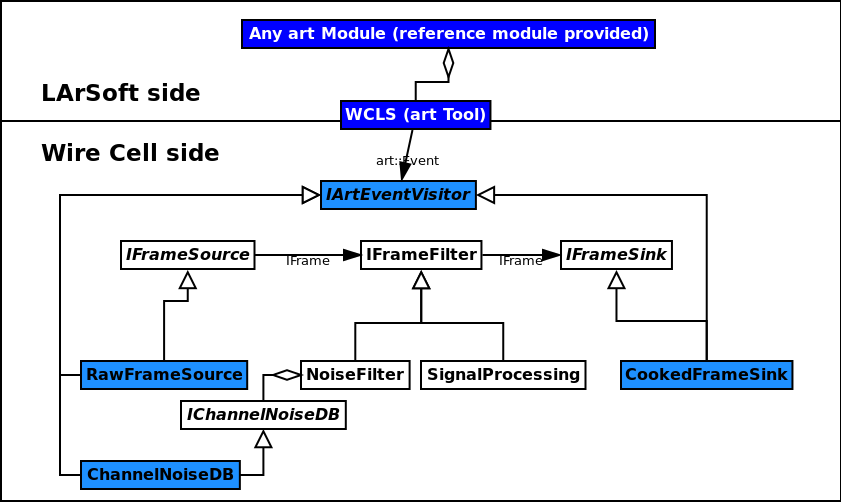
\includegraphics[height=0.8\textheight]{nfsp-integ.pdf}
  \end{center}
\end{frame}

\begin{frame}
  \frametitle{WC/LS Design In Words}
  \begin{itemize}
  \item \texttt{WireCellToolkit\_module} provides reference \textit{art} module.
  \item \texttt{WCLS\_tool} provides \textit{art} Tool interface almost exactly like \texttt{wire-cell} command line interface.
  \item A pure-WCT DFP graph may be rewritten to a WC/LS graph simply by replacing its data sources/sinks with corresponding WC/LS \textbf{converter components}.
    \begin{itemize}\footnotesize
    \item[o] ``visit'' the \texttt{art::Event} before or after module execution.
    \item[o] convert data or provide interface to \textit{art} services.
    \end{itemize}
  \item High-level WCT configuration specified in FHiCL 
    \begin{itemize}\footnotesize
    \item Corresponds to what may otherwise be specified to \texttt{wire-cell} CLI
    \item Typically, a few select ``external variable'' parameters set in FHiCL
    \item Additionally, must specify list of converter components.
    \end{itemize}
  \end{itemize}
\end{frame}


\begin{frame}
  \frametitle{WC/LS Status}
  \begin{itemize}
  \item WCT is now standard for MicroBooNE noise filtering and signal processing.
  \item WCT simulation integrated and tested to consume LArG4 energy depositions, produce raw ADC waveforms.
  \item Multi-APA support added to above to support ProtoDUNE-SP.
  \end{itemize}
\end{frame}

\section{Strategy and Discussion}
\begin{frame}
  \tableofcontents[currentsection,hideothersubsections]
\end{frame}

\begin{frame}
  \frametitle{WCT Strategy For DUNE}
  \begin{enumerate}
  \item Continue to advance algorithms and port to toolkit 
  \item Add support for per-APA processing
    \begin{itemize}\scriptsize
    \item Relatively straight-forward in WCT 
    \item But, need a per-APA ``loop'' all the way to the input file (ie, \textit{art} support).
    \end{itemize}
  \item Leverage WCT design to exploit multi-core platforms and reduce RAM/core.
  \item Understand if multi-core GRID jobs are sufficient for DUNE production data and simulation processing and push into HPC space if not.
  \end{enumerate}

  Some more on each point on following slides.
\end{frame}


\begin{frame}
  \frametitle{Wire-Cell Algorithm Advancement}

  \begin{center}
    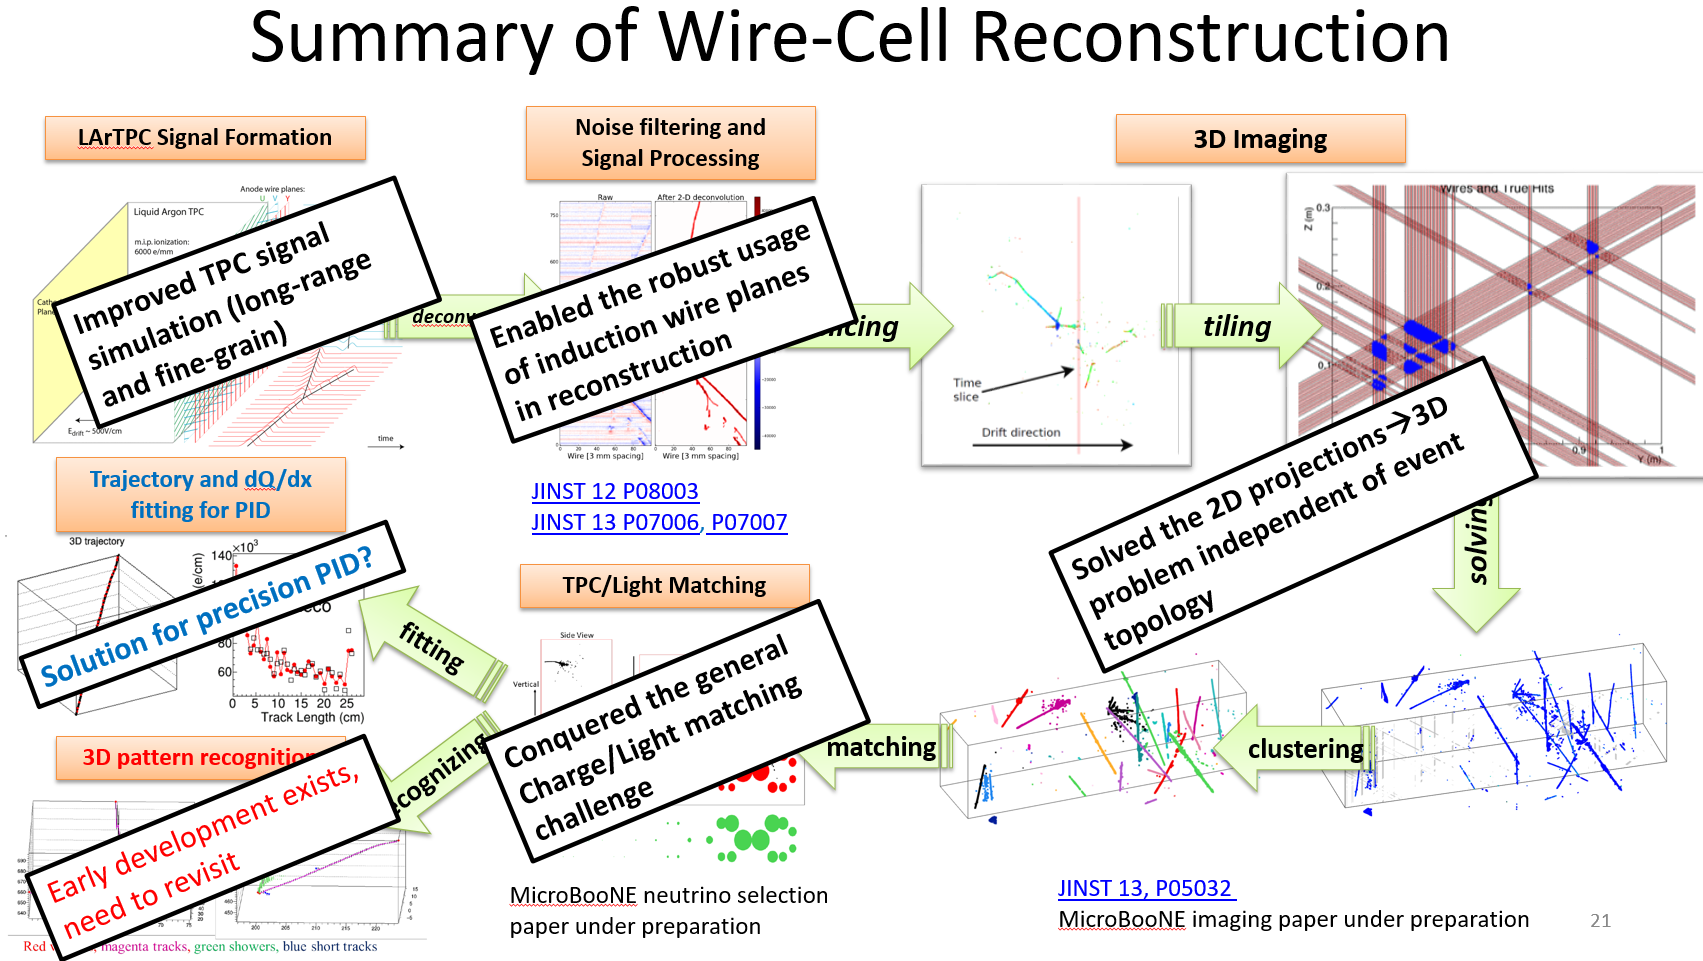
\includegraphics[width=\textwidth,clip,trim=0 0 0 3cm]{summary-of-wc-reco-boxes.png}

    \tiny Xin Qian
  \end{center}

\end{frame}


\begin{frame}
  \frametitle{Porting Prototype Algorithms - 3D Imaging}

  \begin{itemize}
  \item Existing 3D prototype code needs understanding by others (started).
  \item New, more general data model needed (conceptual).
  \item Develop optimized primitive operations (conceptual).
  \item Initiate new eg \texttt{wire-cell-img} package.
  \item Initial port of algorithms should generically support MB, PDSP and others.
  \item Benchmarking, validation, tuning....
  \end{itemize}
  
\end{frame}


\begin{frame}
  \frametitle{Per-APA execution model}
  \begin{itemize}
  \item Full ``event'' in memory already requires substantial RAM
    \begin{itemize}\footnotesize
    \item[o] MicroBooNE/ProtoDUNE-SP easily break the 2GB/core Grid limit.
    \item[o] WCT recently reduced its footprint but still processes whole-event
    \item[o] art's ROOT I/O overhead tends to dominate
    \item[o] 150 DUNE APAs in memory at once is untenable
    \end{itemize}
  \item SigProc output is sparse, expect $\approx10^4$ reduction for DUNE
  \item Input is dense: break processing down to per-APA units.
    \begin{itemize}\footnotesize
    \item[o] WCT can define per-APA pipelines, some work needed.
    \item[o] Ultimately, only matters if \textit{art} loads in $\mathcal{N}$ APAs at once
    \end{itemize}
  \end{itemize}

  Discussion:
  \begin{itemize}\footnotesize
  \item[$\to$] DUNE needs to discuss with \textit{art}/LArSoft experts how to achieve a per-APA ``event'' loop. 
  \item[$\to$] DUNE should configure production jobs to be more selective as to what data types are ``shunted'' input$\to$output.
    \begin{itemize}\scriptsize
    \item Don't carry forward ``dense'' \texttt{RawDigits}.
    \end{itemize}
  \end{itemize}
\end{frame}

\begin{frame}
  \frametitle{protoDUNE WC/LS SigProc memory usage}
  \begin{columns}
    \begin{column}{0.2\textwidth}
      \tiny

      6-APA event

      \vspace{2mm}

      After recent $\approx$ 500 MB reduction inside WCT

      \vspace{2mm}

      \colorbox{lightgray}{\textcolor{red}{ROOT output}}

      \colorbox{lightgray}{\textcolor{orange}{WCT sigproc}}

      \colorbox{lightgray}{\textcolor{yellow}{ROOT input}}

    \end{column}

    \begin{column}{0.4\textwidth}
      \begin{center}
        \tiny Copy all input to output (2GB, 30min).
        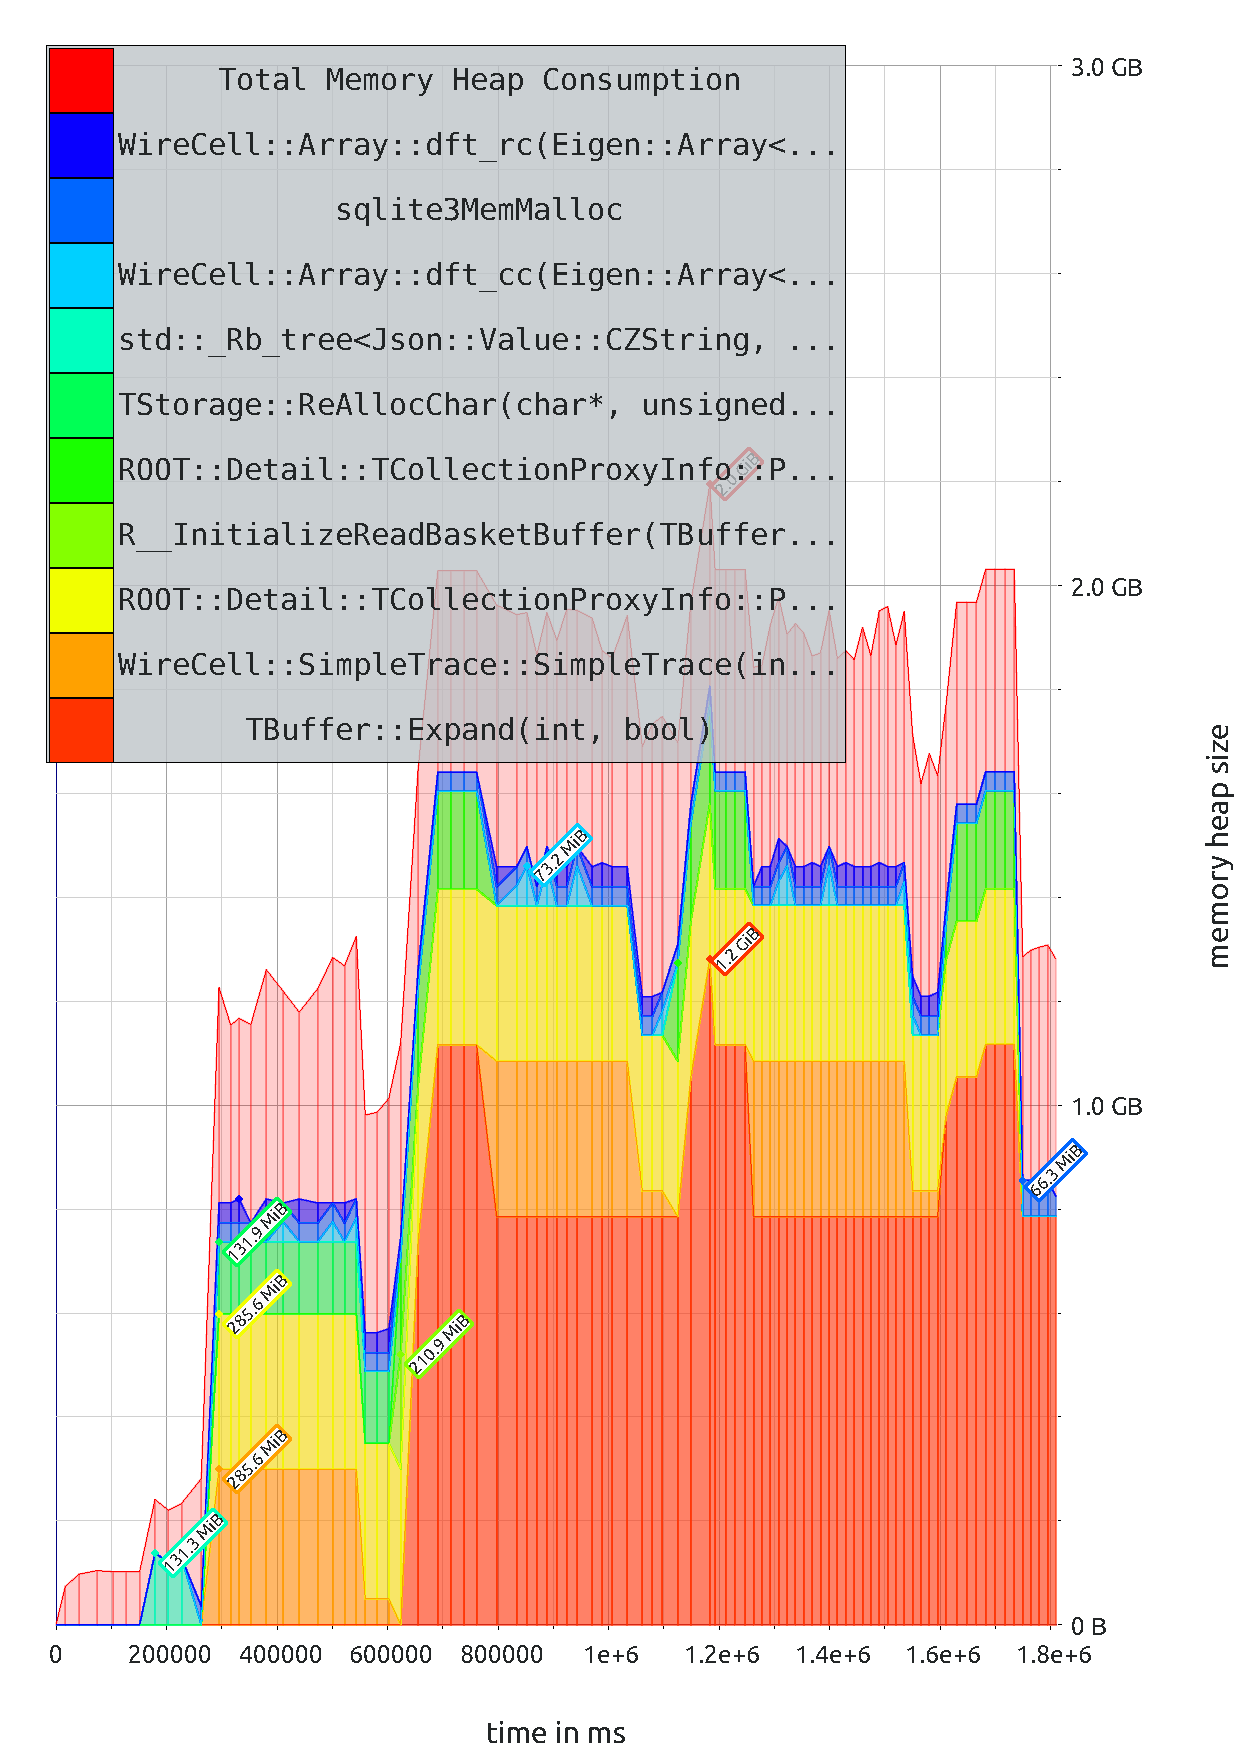
\includegraphics[height=0.8\textheight]{shunt.pdf}    
        
      \end{center}
    \end{column}

    \begin{column}{0.4\textwidth}
      \begin{center}
        \tiny No unneeded I/O copy (1.2GB, 23min).
        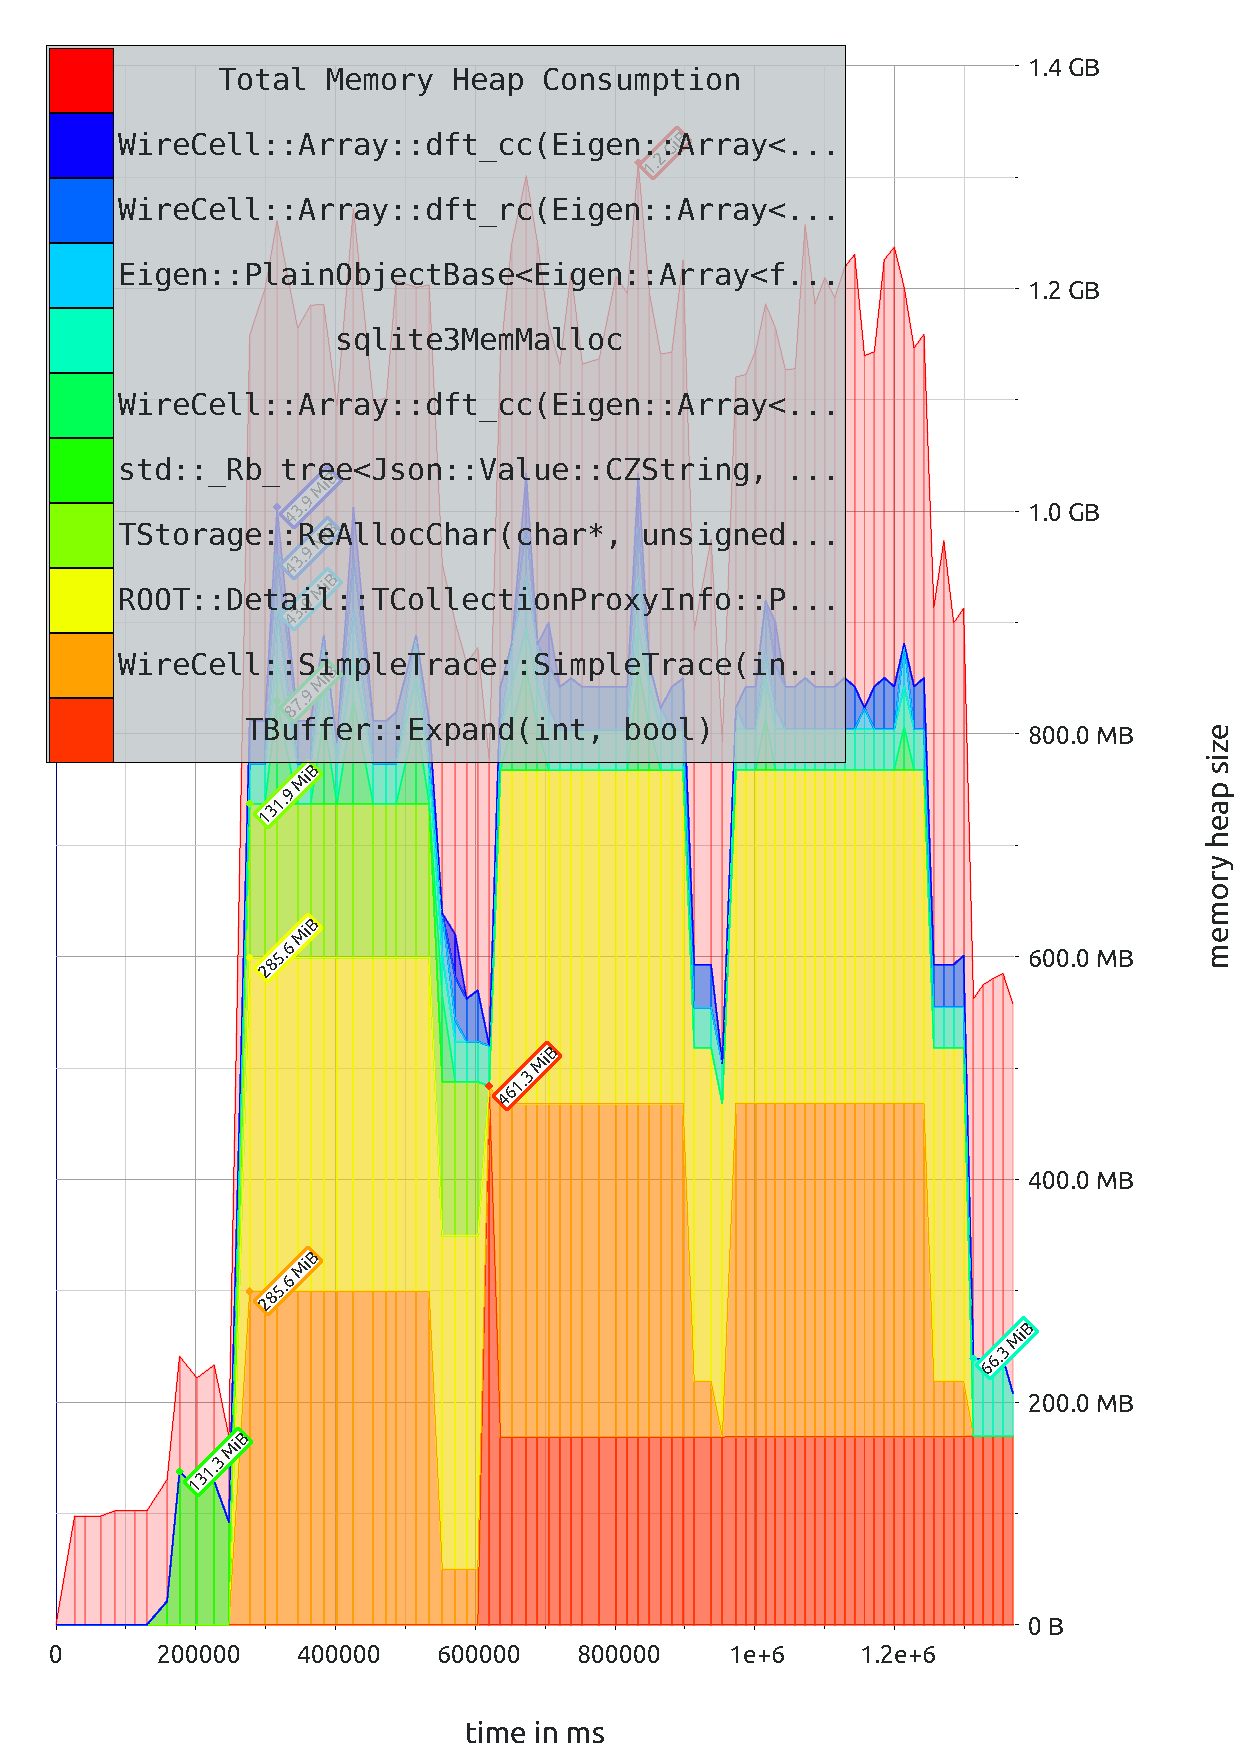
\includegraphics[height=0.8\textheight]{noshunt.pdf}
      \end{center}
    \end{column}
    
  \end{columns}

  \begin{center}
  \end{center}
\end{frame}

\begin{frame}
  \frametitle{Multi-threading}

  \begin{itemize}\footnotesize
  \item WCT has existing TBB-based multi-threaded DFP graph execution engine.
    \begin{itemize}\scriptsize
    \item[o] May be ``trivial'' or maybe surprises.
    \item[+] No mutable ``globals'', \texttt{const} data objects so should be in good shape.
    \item[?] But, many node components exist now and with little care for thread-safety.
    \end{itemize}
  \item Evaluate TBB execution performance and memory usage
  \item Consider adoption/development of alternative engines.
  \item Understand how far we can go on multi-core grid allocation alone.
  \item Test the HPC waters.
  \end{itemize}
  
\end{frame}

\begin{frame}
  \frametitle{Thoughts on \textit{art} Multi-threading}
  \begin{itemize}\footnotesize
  \item \textit{art} is multi-threaded but ``only'' at the module/path level, 
    \begin{itemize}\scriptsize
    \item[o] This useful feature seems not yet exploited by the experiments. 
    \item[$\to$] DUNE should try it!
    \item[?] Only useful to the extent that module paths are actually parallel.
    \end{itemize}
  \item MT success and per-APA execution are linked.
    \begin{itemize}\scriptsize
    \item[o] Ideally, we want concurrent, per-APA pipelines.
    \item[o] These will require ``event'' level synchronization at least at job output.
    \end{itemize}
  \item Must treat parallelism ``holistically''
    \begin{itemize}\scriptsize
    \item[o] A highly parallel module (eg WCT) in an otherwise roughly serial \textit{art} job wastes CPU.
    \item[$\to$] See if \textit{art} team can add pipelining (multiple events ``in flight'').
    \item[o] WCT components may be pipelined ``for free'' depending on the execution engine.
    \item[o] BNL PAS group's ``event server'' technique may also be useful?
    \end{itemize}
  \end{itemize}
\end{frame}

\begin{frame}
  \frametitle{Multi-Core Grid vs HPC}
  It's not yet clear to me if DUNE \textbf{really} needs HPC. 
  \begin{itemize}
  \item[?] Would achieving good CPU efficiency on Grid be enough?
    \begin{itemize}\scriptsize
    \item How much CPU-years does DUNE need?
    \end{itemize}
  \item[-] Supporting HPC will take work:
    \begin{itemize}\scriptsize
    \item[o] must greatly reduce RAM/core, support fine(ish) grain MT, 
    \item[o] understand and obey special software environments (I'm told: ``no ROOT'') 
    \item[o] infrastructure, data ingest/egress, databases, security issues.
    \item[o] in some cases deal with ``unusual'' CPU architecture and OS.
    \end{itemize}
  \item[+/-] We would be minor player on HPC
  \item[++] HPC power could open up new algorithms
    \begin{itemize}\scriptsize
    \item[?] do we make the support effort just ``in case''?
    \end{itemize}
  \end{itemize}

\end{frame}

\end{document}

